\documentclass[10pt,pdf,hyperref={unicode}]{beamer}

\usepackage{float}
\usepackage{amsmath}
\usepackage{amsfonts}
\usepackage{bbm}

% русский текст в формулах?
\usepackage{mathtext}

% русский
\usepackage[T2A]{fontenc}
\usepackage[english]{babel}
\usepackage[utf8]{inputenc}

% рисунки
\usepackage{graphicx, caption, subcaption}

\usetheme{CambridgeUS}

\usepackage{csquotes}
\usepackage[backend=bibtex]{biblatex}
\bibliography{biblio}

% ?
\setbeamertemplate{frametitle}[default][center]

\addtobeamertemplate{navigation symbols}{}{%
\usebeamerfont{footline}%
\usebeamercolor[fg]{footline}%
\hspace{1em}%
\large\insertframenumber/\inserttotalframenumber
}

\newcommand{\mytitle}[1]{\color{blue}{\textbf{#1}}}

\newcommand{\lb}{\left(}
\newcommand{\rb}{\right)}

\begin{document}

\begin{frame}{\center\mytitle{\Large Quantum scattering with a spherically symmetric potential}}
\begin{table}[]
\flushright
\begin{tabular}{r}
\large Finenko Artoum \\
\large 515 group
\end{tabular}
\end{table}
\vfill
\center
\today
\end{frame}

\begin{frame}{Scattering phenomena: background \footfullcite{rodberg}} 

\begin{columns}[T] % align columns

\begin{column}{.48\linewidth}
	\begin{itemize}
		\item In an idealized scattering experiment, a sharp beam of particles (A) of definite momentum $\mathbf{k}$ are scattered from a localized target (B).
		\item As a result of collision, several outcomes are possible:
			\begin{gather}
				A + B \longrightarrow 
				\left\{
				\begin{aligned}
					A + B \quad \quad \text{elastic} \\
					\left.
					\begin{aligned}
						A + B^* \\
						A + B + C 
					\end{aligned}
					\right\} \quad \quad \text{inelastic} \\
					C \quad \quad \text{absorption}
				\end{aligned}	
				\right. \notag
			\end{gather}

	\end{itemize}
\end{column}
\begin{column}{.48\linewidth}
	\vspace*{-1cm}
	\begin{figure}
		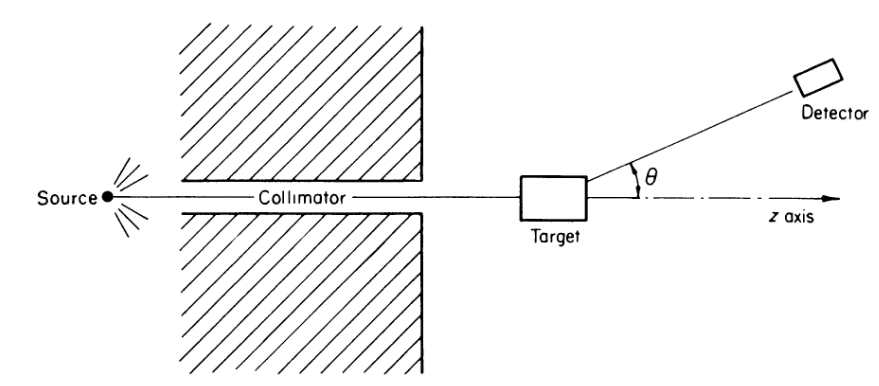
\includegraphics[scale=0.2]{./pictures/experiment.png}
		\caption{A schematic representation of a standard scattering experiment} 
	\end{figure}
\end{column}
\end{columns}
\end{frame}

\begin{frame}{Scattering phenomena: differential and total cross section}
\begin{itemize}
	\item Detector measures the number of particles per unit time, $N d\Omega$, scattered into an element of solid angle $d\Omega$ in direction $(\theta, \phi)$.
	\item The number is proportional to the incident flux of particles, $j_\text{inc}$, defined as the number of particles per unit time crossing a unit area normal to direction of incidence.
	\item Collisions are characterised by the \textbf{differential cross section} defined as the ratio of the number of particles scattered into direction $(\theta, \phi)$ per unit time per unit solid angle, divided by the incident flux
	\begin{gather}
		\frac{d\sigma}{d\Omega} = \frac{N}{j_\text{inc}} \notag
	\end{gather}
	\item From the differential, we can obtain the \textbf{total cross section} by integrating over all solid angles
	\begin{gather}
		\sigma = \int \frac{d\sigma}{d\Omega} d\Omega = \int\limits_0^{2\pi} d \phi \int\limits_0^\pi \frac{d\sigma}{d\Omega} \sin \theta d\theta \notag
	\end{gather}
\end{itemize}
\end{frame}


\begin{frame}{Lectures recap}
	The Hamiltonian for a system of two interacting particles
	\begin{gather}
		\hat{H} = \frac{\mathbf{P}_A^2}{2 m_A} + \frac{\mathbf{P}_B^2}{2 m_B} + V_{AB} \notag
	\end{gather}
	Separating out the motion of the center of mass
	\begin{gather}
		\mathbf{r} \equiv \mathbf{r}_A - \mathbf{r}_B, \quad \mathbf{R} \equiv \frac{m_A \mathbf{r}_A + m_B \mathbf{r}_B}{m_A + m_B} \notag \\
		\left[ -\frac{\hbar^2}{2M} \nabla_R^2 - \frac{\hbar^2}{2\mu} \nabla_r^2 + V(r) \right] \Psi(\mathbf{r}_A, \mathbf{r}_B) = E \Psi(\mathbf{r}_A, \mathbf{r}_B), \notag
	\end{gather}
	where 
	\begin{gather}
		M = m_A + m_B, \quad \mu = \frac{m_A m_B}{m_A  + m_B} \notag
	\end{gather}
\end{frame}

\begin{frame}{Lectures recap II}
	It permits a separation of the variables $\mathbf{R}$ and $\mathbf{r}$
	\begin{gather}
		\Psi(\mathbf{r}_A, \mathbf{r}_B) = \Phi(\mathbf{R}) \psi(\mathbf{r}) \notag \\
		-\frac{\hbar^2}{2M} \nabla^2_R \Phi(\mathbf{R}) = E_\text{cm} \Phi(\mathbf{R}) \notag \\
		\left\{ -\frac{\hbar^2}{2\mu} \nabla^2 + V(r) \right\} \psi(\mathbf{r}) = E_\text{rel} \psi(\mathbf{r})
	\end{gather}
	where 
	\begin{gather}
		E = E_\text{cm} + E_\text{rel}
	\end{gather}
\end{frame}

\begin{frame}{Stationary scattering theory}
	Asymptotically $\psi$ must consist of an incoming wave and an outgoing spherical wave centered about the origin of the scattering field. The amplitude of the scattered wave depends on two angles $\theta$ and $\phi$. 
	\begin{gather}
			\psi(\mathbf{r}) \xrightarrow[r \rightarrow \infty]{} \exp \lb i \lb \mathbf{k} \cdot \mathbf{r} \rb \rb + \frac{\exp \lb i k r \rb}{r} f(\theta, \phi) = \psi_0 + \psi_s \notag
	\end{gather}
	Asymptotic behavior of the cross sections can be obtained by considering the particle flux. The particle flux density is
	\begin{gather}
		\mathbf{j} = -\frac{i \hbar}{2 \mu} \lb \psi^* \nabla \psi - \psi \nabla \psi^* \rb \notag
	\end{gather}
	Incident plane wave $\psi_0$ and scattered wave $\psi_s$ yield corresponding flux densities
	\begin{gather}
		\mathbf{j}_0 = \frac{\hbar \mathbf{k}}{\mu}, \quad
		\mathbf{j}_s  = \frac{\hbar \mathbf{k}}{\mu r^2} | f(\theta, \phi) |^2. \notag
	\end{gather}
	Following the definition of the differential scattering cross section
	\begin{gather}
			\frac{d\sigma}{d \Omega} = \frac{\text{particle flux scattered into unit solid angle} \, d\Omega}{\text{incident particle flux density}} = |f(\theta, \phi)|^2 \notag
	\end{gather}
\end{frame}

\begin{frame}
	For a spherically symmetric potential, the solution of the Schroedinger equation can always be written as 
	\begin{gather}
		\psi(\mathbf{r}) = \sum_{l = 0}^\infty \sum_{m = -l}^l A_{lm} \frac{u_l(r)}{r} Y_l^m(\theta, \phi) \notag
	\end{gather}
	where $u_l$ satisfies the radial Schroedinger equation
	\begin{gather}
		\left\{ \frac{\hbar^2}{2\mu} \frac{d^2}{dr^2} + \left[ E - V(r) - \frac{\hbar^2 l(l+1)}{2 \mu r^2} \right] \right\} u_l(r) = 0.
	\end{gather}

	Outside the well, the solution $u_l$ can be written as a linear combination of \textit{spherical Bessel} and \textit{spherical Neumann} functions of order l:
	\begin{gather}
			u_l(r) = A r j_l(k r) + B r n_l(k r), \quad k = \sqrt{2 \mu E}{\hbar}, \notag \\
		\text{where} \quad j_l(x) = (-x)^l \lb \frac{1}{x} \frac{d}{dx} \rb^l \frac{\sin x}{x}, \notag \\
		\text{and} \quad n_l(x) = - (-x)^l \lb \frac{1}{x} \frac{d}{dx} \rb^l \frac{\cos x}{x}. \notag 
	\end{gather}
\end{frame}

\begin{frame}
		$u_l$ approaches a sine-wave form for large $r$ and the phase of this wave is determined by $\delta_l$ \footfullcite{LL}
	\begin{gather}
		u_l(r) \sim \sin (kr - l \pi / 2 + \delta_l). \notag
	\end{gather}
	Phase-shifts $\delta_l$ determine scattering amplitude $f(\theta)$ by relation 
	\begin{gather}
		f(\theta) = \frac{1}{2 ik} \sum_{l = 0}^\infty (2l + 1)(S_l - 1) P_l(\cos \theta), \quad S_l = \exp \lb 2 i \delta_l \rb. \notag
	\end{gather}
	Substituting previous relation into definition of the total cross section we get
	\begin{gather}
		\sigma = \frac{4 \pi}{k^2} \sum_{l = 0}^\infty (2l + 1) \sin^2 \delta_l . \notag
	\end{gather}
\end{frame}

\begin{frame}{Numerical procedure for calculating cross sections \footfullcite{thijssen}}
		Select some definite value of energy $E$ and for all values of angular momentum $l$ from $0$ to $l_\text{max}$:
\begin{enumerate}
	\item Integrate the radial Schroedinger equation to some $r_\text{max}$ value
	\item Match the numerical solution with spherical Bessel and Neumann functions to determine phase shift $\delta_l$
	\item Calculate contribution to cross section 
\end{enumerate}
\end{frame}

\begin{frame}{Numerov's method for the radial Schroedinger equation}
	Define auxiliary function 
	\begin{gather}
		F(l, r, E) = V(r) + \frac{\hbar^2 l(l + 1)}{2 \mu r^2} - E \notag
	\end{gather}
	so that the radial Schroedinger equation now reads
	\begin{gather}
		\frac{\hbar^2}{2 \mu} \frac{d^2}{dr^2} u(r) = F(l, r, E) u(r). \notag
	\end{gather}
	Numerov's algorithm makes use of the special structure of this equation to solve it with an error of order $h^6$. For $\hbar^2/2\mu \equiv 1$ it reads:
	\begin{gather}
		\omega(r + h) = 2 \omega(r) - \omega(r - h) + h^2 F(l, r, E) u(r) \notag \\
		u(r) = \lb 1 - \frac{h^2}{12} F(l, r, E) \rb^{-1} \omega(r). \notag
	\end{gather}
\end{frame}

\begin{frame}{Interaction potential}
	Model system: H-Kr. The two-atom interaction potential is often modelled by the Lennard-Jones potential of the following form:
	\begin{gather}
			V_{\text{LJ}}(r) = \varepsilon \left[ \lb \frac{\rho}{r} \rb^{12} - 2 \lb \frac{\rho}{r} \rb^6 \right], \quad \varepsilon = 5.9 \text{meV}, \quad \rho = 3.57 \textup{\AA}. \notag 
	\end{gather}
	\vspace*{-1cm}
	\begin{figure}
		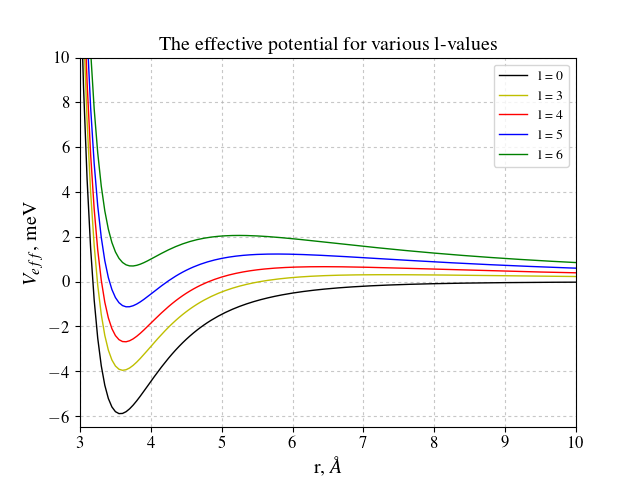
\includegraphics[scale = 0.35]{../numerov_LJ/pictures/effective_potential.png}
	\end{figure}
\end{frame}

\begin{frame}{}
	The first two points can be calculated in the following way, assuming the asymptotic form for $r \rightarrow 0$:
	\begin{gather}
		\frac{\hbar^2}{2\mu} \frac{d^2}{dr^2} u(r) \approx \varepsilon \lb \frac{\rho}{r} \rb^{12} u(r), \notag \\
		u(r) \approx \exp \lb - \sqrt{\frac{2 \mu \varepsilon \rho^{12}}{25 \hbar^2}} r^{-5} \rb . \notag 
	\end{gather}

	Matching the numerical solution to asymptotic solution is done via two point method
	\begin{gather}
		\tan \delta_l = \frac{K j_l^{(1)} - j_l^{(2)}}{K n_l^{(1)} - n_l^{(2)}} \quad \text{with} \quad K = \frac{r_1 u_l^{(2)}}{r_2 u_l^{(1)}}. \notag
	\end{gather}
\end{frame}

\begin{frame}
	\begin{figure}
		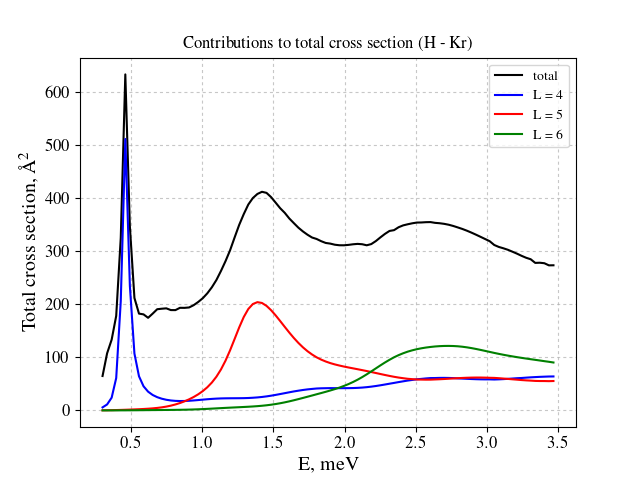
\includegraphics[scale=0.5]{../numerov_LJ/pictures/contributions.png}
	\end{figure}
\end{frame}

\begin{frame}{Experimental results\footfullcite{toennies1979}}
	\vspace*{-0.2cm}
	\begin{figure}
		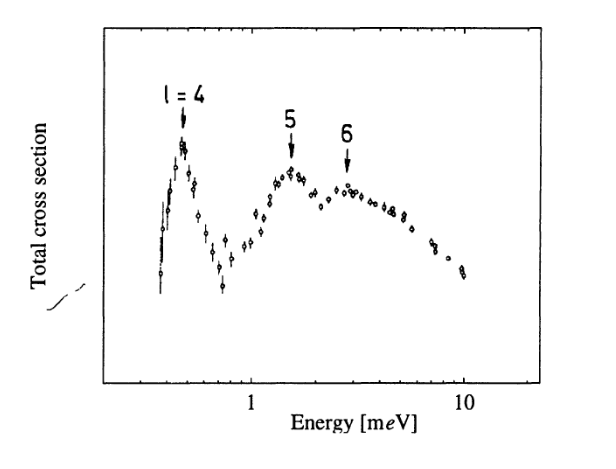
\includegraphics[scale=0.4]{../numerov_LJ/pictures/experiment.png}
	\end{figure}
\end{frame}

\begin{frame}{Radial wavefunctions in the vicinity of the resonance L = 4}
	\vspace*{-1.3cm}
	\begin{figure}
		\hspace*{-2.5cm}
		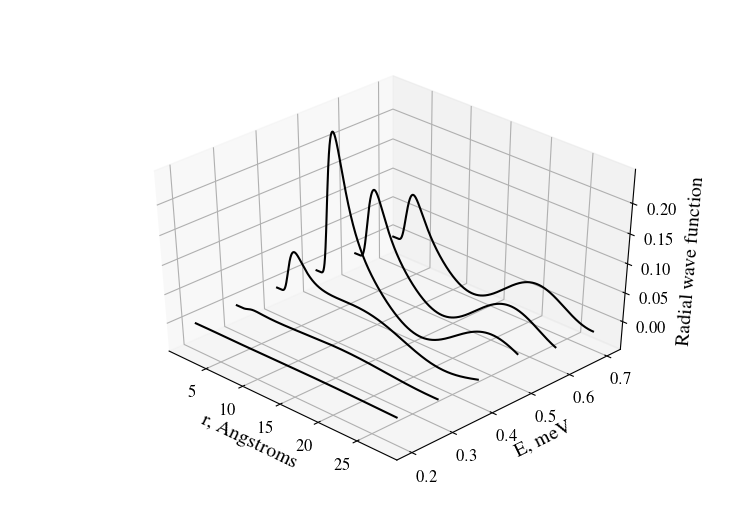
\includegraphics[scale=0.5]{../numerov_LJ/pictures/l_4_wavefunctions.png}
	\end{figure}
\end{frame}

\end{document}


